\chapter{Static Computational Optical Undersampled Tracker}\label{chap:Scout}

\section{Motivation for the Static Computational Undersampled Tracker}

In large-area persistent surveillance, traditional \gls{isomorphic} sensing systems which are based on the Shannon-Nyquist sampling theorem must acquire, process, store, and transmit large amounts of data to achieve high spatial and temporal resolution. These sensors are often on airborne or orbiting platforms which leads to a large \acrfull{swap-c}. However, if the application is specific to only tracking moving targets, the information content in the signal-of-interest is relatively low compared to the data in the measurement. Furthermore, one can design a sensor which measures the temporally varying aspects of the target to promote \gls{sparsity}. This intuitively leads one to turn to techniques based on \gls{compressive sensing}. This chapter discusses a simple low cost optical tracking architecture based on compressive sensing techniques, called the \acrfull{scout}, to address the challenges of traditional target tracking. 

Experimental demonstrations of \gls{compressive sensing} for imaging are often very general and reconstruct the entire object scene or spatial-temporal datacube. For example, the \gls{cacti} uses a piezo linear stages to translate a psuedo-random binary coded aperture during a single \gls{fpa} exposure and attempts to reconstruct temporal varying object scenes \cite{llull2013coded}. A compressive imager based on a rotating cylindrical lens and \gls{fpa} measured scene data using an optical Radon transforms in a sequential manner to reconstruct an object scene \cite{evladov2012progressive}. While these schemes demonstrate the progress that experimentalists have made towards compressive imaging, they emphasize reconstructing high dimensional data and therefore will require another post-processing step to extract task-specific information. Furthermore, this data will then need to be compressed again for storage or transmission. 

The single pixel camera, discussed in \Cref{sec:multiplexingtocompressivesensing}, uses a \acrfull{dmd} to measure in any arbitrary basis, but must do so over many time-sequential measurements \cite{duarte2008single}. Each measurement is an integrated point-by-point multiplication of the scene locations with the \gls{dmd} array values. For temporally static scenes, this architecture allows an arbitrarily long exposure time (within the limit of detector saturation) to increase the \gls{snr} for each measurement. However, with temporally varying scenes it needs to record all the projections for each frame before the object moves.  Increasing the rate at which projections are made is possible, but this reduces exposure time and \gls{snr}. One way to overcome this is by implementing a parallel architecture of single pixel cameras, each with a different projection, see \Cref{fig:parallelcsimager2}. Clearly this will significantly increase the \gls{swap-c} of the architecture. Another issue with fully parallel architecture, is that each camera will have a different entrance pupil, producing a certain amount of parallax. One issue many computational sensor designs must deal with is over multiplexing. All real optical \gls{adc} devices have a certain amount of dynamic range in which linearity is valid. As the amount of light that is recorded increases, the amount of dynamic range being used fills up. In the limit of a single detector element this can be a serious issue. 

An architecture dedicated to target tracking rather than full object scene reconstruction, can significantly ameliorate these design trade-offs. We developed the \acrfull{scout} with the goal that measurements must be acquired ``single-shot'' using a conventional \gls{fpa} \cite{townsend2012static, poon2012advances}. The \gls{scout} system is an important step toward practical low-cost computational sensing for optical imaging. The system enables parallel ``single-shot'' acquisition of compressed, task-specific sensing oriented data, using a static (no moving parts) architecture.

A related static approach uses optical Radon projections \cite{kashter2012optical}. This instrument relies on a several cylindrical lenses to integrate the optical intensity from object plane along a lines on the \gls{fpa}. The number of detector elements is much less than the native dimensionality of the object scene. For a single moving point in the field-of-view two perpendicular Radon projections is enough to compute the change from frame to frame. However, the researchers found heuristically that $4$ cylindrical lens are better for reconstructing the change information for an scene that included up to $10$ moving objects, called movers. However, this approach is more complicated in terms of opto-mechanics than the \gls{scout} to implement since it requires mounting cylindrical lenses in a certain configuration. 

In this chapter, I will discuss the \gls{scout} architecture, described in detail in \Cref{sec:ScoutArchitecture}, which uses a defocused imaging system with two binary amplitude masks. The \gls{fpa} samples at a much lower resolution than resolution of the object scene. While other compressive imaging systems have to reconstruct entire images, the \gls{scout} only reconstructs frame-to-frame differences. As a result the \gls{scout}  requires significantly less bandwidth to transmitted compressively sampled data. 

 

\begin{figure}
	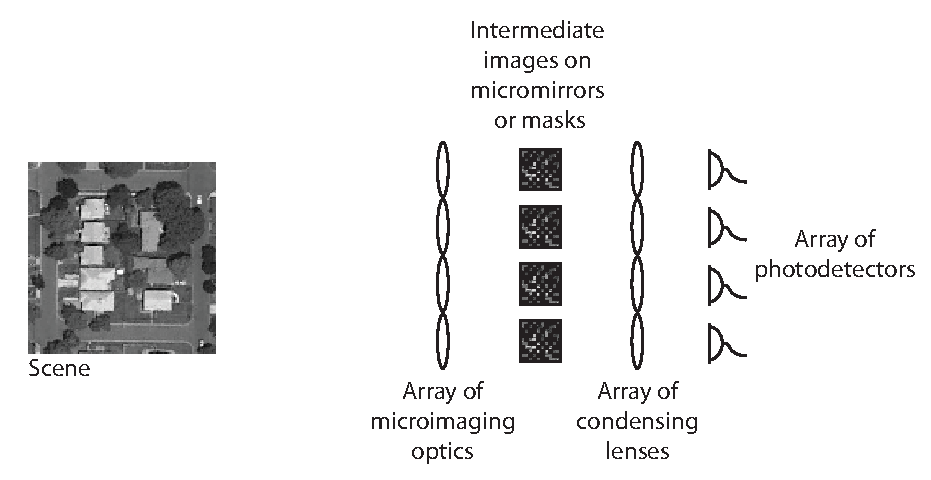
\includegraphics[scale=0.9]{parallelcsimager2}
	\captionof{figure}[The architecture of a hypothetical parallel single pixel camera to capture simultaneous projections.]{An example of a typical parallel optical CS architecture. Capturing $N_m$ simultaneous projections requires using $N_m$ spatial light modulators or masks and $N_m$ detector elements.}
	\label{fig:parallelcsimager2}
\end{figure}




\section{SCOUT Architecture}\label{sec:ScoutArchitecture}


The \gls{scout} architecture is designed to capture the differences of dynamic scenes while avoiding the hardware scaling issues of the aforementioned \gls{compressive sensing} imaging architectures. The trade-off for the ability to measure parallel projections is the lost flexibility to implement arbitrary projections using an \gls{slm}. However, rather than fully designing the projections themselves, I describe a process for optimizing the optical instrument  in \Cref{sec:ScoutSimulations}. Previous prototypes of the \gls{scout} architecture are described in \cite{stenner2010static, rivenson2010single}. 

The \gls{scout} system takes measurements that are both compressive and multiplexed: The number of measurements must be fewer than the number of scene locations $N_m \ll N$, and each measurement must contain information about many scene locations. In this architecture, the number of measurements is the number of pixels in the \gls{fpa}. Intuitively this means that the system matrix must exhibit a many-to-few mapping from scene locations to \gls{fpa} elements. 

The \gls{scout} architecture is shown in \Cref{fig:scoutArchitecture}. In this architecture the \gls{multiplexing} occurs in the spatial domain by mapping multiple object scene locations to only a few detector pixels. To accomplish this, we created a structured blur. This blur allows the light to be spread to several pixels on the \gls{fpa}. The most straightforward way to achieve a blur is by defocusing the image so that the \gls{psf} is broad, spanning many pixels. Since the number of \gls{fpa} pixels are less than the object scene resolution, this process is compressive. Like any aberration, defocus significantly reduces contrast of high spatial frequencies, so the measurements will poorly conditioned for reconstruction. Therefore, we created high-frequency structure in the \gls{psf} by using two pseudo-random binary occlusion masks. Each mask is placed at different positions between the lens and the sensor. The separation between masks results in spatially varying point-spread function. 

\begin{figure}
	\includegraphics[scale=1.2]{scoutArchitecture}
	\captionof{figure}[The SCOUT architecture.]{A diagram of the \gls{scout} architecture. A lens projects light through a pair of binary occlusion masks onto a low-resolution sensor which is defocused from the nominal image plane. This creates a spatially multiplexed shift-variant PSF incident on the \gls{fpa}.  }
	\label{fig:scoutArchitecture}
\end{figure}

As with many computational sensing architectures, the forward model is described by 
%
\begin{equation}
	\mb{g} = \mb{H} \mb{f} + \mb{e}
	\label{eq:scoutgHf}
\end{equation}
%
In this equation, the 2-dimensional object scene with resolution $ R_x \times R_y$ elements, is lexicography reordered into a $N \times 1$ column vector, $\mb{f}$. Similarly, the measurement vector $\mb{g}$ is an $N_m \times 1$ vector representing a 2-dimensional measurement with a $ R_x \times R_y$ matrix which represents the low resolution measurement. The detector noise is represented by the $ N_m \times 1 $ vector $\mb{e}$.

The system matrix $\mb{H}$ is thus $N_m \times N $ matrix, where $N_m \ll N$ in order to the system to be considered compressive. The $n^{th}$ column of $\mb{H}$ describes the \gls{psf} of the $n^{th}$ image element. In other words, each column of the system matrix is the low resolution read-out of the \gls{fpa}. Whereas the $m^{th}$ row of $\mb{H}$ describes the weights of each scene location’s contribution to the $m^{th}$ measurement. In this way, the resulting system matrix $\mb{H}$ demonstrates that the \gls{scout} is a spatially variant optical system and presents a block structure, as seen in the example shown in \Cref{fig:scoutSysResponse}.

\begin{sidewaysfigure}
	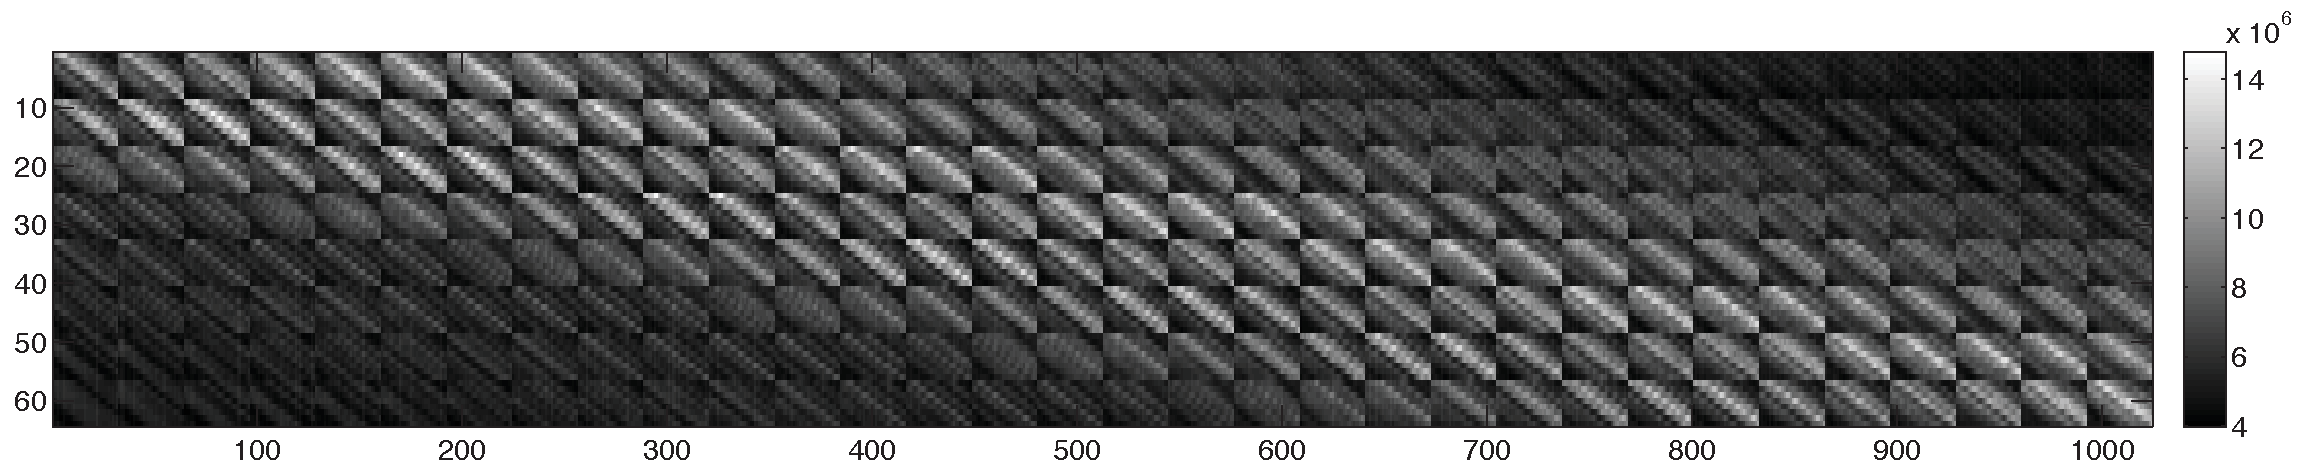
\includegraphics[scale=0.65]{scoutSysResponse}
	\captionof{figure}[An example of the system matrix of the \gls{scout}.]{An example of an experimentally measured of the system matrix of the \gls{scout} system. The approximate block-Toeplitz structure is clearly evident, as is the deviation from the Bernoulli or Gaussian ensembles typically considered in CS treatments. }
	\label{fig:scoutSysResponse}
\end{sidewaysfigure}

Like any compressive sensing technique, the assumption of a sparse or compressible representation for the signal-of-interest is required. While light from every point in the object scene is recorded, only the differences between successive measurements scenes are processed, stored, and transmitted to the base station
%
\begin{equation} 
\begin{split}
	\mb{g}_1 &= \mb{H} \mb{f}_1 + \mb{e}_1 \\
	\mb{g}_2 &= \mb{H} \mb{f}_2 + \mb{e}_2
\end{split}
\end{equation}
%
\begin{equation}
	\Delta \mb{g} = \mb{g}_2 - \mb{g}_1 = \mb{H} \ap{ \mb{f}_2 - \mb{f}_1 } + \mb{e}_2 - \mb{e}_1 
\end{equation}
%
Where the subscripts represent the readout $k^{th}$ readout from the \gls{fpa}. Assuming that the background is relatively static between \gls{fpa} exposures, the differences are sparse. Thus the signal-of-interest $\Delta \mb{f}$ is sparse. Note that in order to achieve sparsity, there is a trade-off, the system records two exposures and therefore two noise realizations. Since the forward model is linear, the frame differences can be calculated in the measurement basis and subsequently reconstructed in the spatial domain. A dot with a negative value indicates the previous location and a positive value indicates the current new location. 

Referring back to the diagram of the \gls{scout} architecture shown in \Cref{fig:scoutArchitecture}. The object distance is much larger than the focal length of the lens so image of the scene occurs approximately one focal length from the lens $f_E$. The \gls{fpa} is placed some distance $d_{im}$ from the focal plane thus the total distance from the lens to the \gls{fpa} is $f_E + d_{im}$. Two binary occlusion masks, mask 1 and mask 2, are placed at distances $d_1$ and $d_2$ from the sensor. Mask 1 and 2 have associated fill factors $F_1$ and $F_2$ and pitch $p_1$ and $p_2$, respectively. 


\section{Calibration}\label{sec:ScoutCalibration}

The system response matrix is determined experimentally by measuring the point spread function of each scene location one at a time, as discussed in detail in \Cref{sec:ScoutCalibration}


Remember that an isomorphic sensor is represented by the identity matrix. In comparison,  in the \gls{scout}, the spatially varying blurred \gls{psf} leads to an approximate block-Toeplitz structure for the system matrix, with approximate Toeplitz structure within individual blocks due to the shifting \gls{psf}. This circulant structure is modified by random variations corresponding to the differing projections created by the two masks. 

As I mentioned in \Cref{chap:Formalism}, random coding has several theoretical properties that make them useful for compressive sensing. There has been some research work to investigate system matrices with Toeplitz and circulant structure \cite{bajwa2007toeplitz, rauhut2009circulant, romberg2009compressive}, however there has been relatively little work published discussing the approximately block-Toeplitz structure that naturally arises in optical systems such as \gls{scout} and theoretical guarantees like the ones force random coding. Two exceptions are \cite{sebert2008toeplitz, liu2008sparsesense}, which provide both theoretical evidence for the viability of CS system matrices with block-Toeplitz structure.


\section{Optimizing the Reconstruction}\label{sec:ScoutSimulations}

While the \gls{scout} lacks the ability to implement arbitrary measurement codes, we are able to adjust various physical parameters of the system such as defocus distance and mask fill factor to minimize reconstruction error. Adjusting each parameter in the actual prototype requires too much time, a more practical approach is to simulated the \gls{scout} architecture was used to evaluate theoretical performance and find values for design parameters, such as defocus distance or mask fill factor, in order to minimize reconstruction errors. In this section we discuss the optical model and the reconstruction technique used, define our tracking-specific reconstruction error metric, then explain how the simulation informed our choice of design parameters.

\subsection{Simulating a SCOUT System}

We developed a paraxial ray based simulation for the \gls{scout}. The simulation allows us to model the effects on the scene as light travels through the lens and two masks onto the detector plane. The lens is modeled as a single thin lens with transmittance function $t_f$ and the two masks have transmittance functions $t_1$ and $t_2$. From calibration measurements, the mask has a transmittances of $0$ where the mask is black and $0.88$ where the mask is clear. The lateral magnification of the scene and the two masks is calculated using similar triangles.

A simulated calibration occurs, in other words the simulation records the $r_x \times r_y$ PSF from each scene location in order to obtain the system matrix $\mb{H}$. Once $\mb{H}$ is known, we use it to simulate the low resolution measurements, $\mb{g}$, of the higher resolution scenes, $\mb{f}$. Subsequent simulated measurements are subtracted to find $\Delta g$. 

Several assumptions are made in the simulation. We assumed a thin lens approximation for the lens. We also did not add any noise.


\subsection{ $\ell_1$ regularized Least Squares Minimization}

Given $\Delta \mb{g}$ and $ \mb{H} $, the reconstruction algorithm finds an estimate, denoted $ \Delta f $, of the original scene’s sparse difference frames. I used the software package for MATLAB \texttt{ l1\_ls } function \cite{kim2007interior} which is an $ \ell_1 $ regularized \gls{ls} minimization algorithm, which is discussed in \Cref{sec:compressiveSesing}.  

\subsection{Quantifying Reconstruction Error}

The \gls{mse} error metric is not suitable for our application because it weights all errors equally. For the task of motion tracking we classify errors into three types. A false positive occurs when the estimate shows an object where there is none. A false negative occurs when the estimate fails to show an object where one exists. As shift error occurs when an object is being tracked but appears in the wrong location. We develop a custom tracking error metric that weighs false negatives and false positives more than shift errors. This is because false negatives and false positives indicate a serious failure in the motion tracking task, while shift errors are less serious. We define tracking error as

\begin{equation}
	P = \frac{ | \mb{a}   \otimes \mb{\epsilon} |}{2N_{mv}}
	\label{eq:scoutErrorMetric}
\end{equation}
%
where
%
\begin{equation}
	\mb{a} = 
	\begin{bmatrix}
	    1/9 & 1/9 & 1/9 \\
	    1/9 & 1/9 & 1/9 \\
	    1/9 & 1/9 & 1/9 
	\end{bmatrix}
\end{equation}
%
where the error $\mb{\epsilon}$ is the difference between the true and reconstructed difference frames
%

\begin{equation}
	\mb{\epsilon} = \Delta \mb{f} - \Delta \mbh{f}
\end{equation}
%
and $N_{\text{mv}}$ is the number of movers in the scene. To reduce the penalty for one-pixel shift errors, the error frame is convolved with a three pixel averaging kernel $\mb{a}$. The absolute value is taken in order to count positive and negative errors equally, and the error is divided by $2N_{mv}$ to make the metric independent of the number of movers. 

\subsection{Optimizing Optical System Parameters}

Now that I have explained the simulation and the custom error metric for tracking error I can finally begin to discuss how we optimized some of the parameters to reduce the reconstruction error. Both the simulation and experimental study demonstrates a relationship between mask position and pitch: the track error is very sensitive to the \emph{projected} mask pitch on the \gls{fpa}. Furthermore, increasing the mask seperation reduced tracking error, generating a highly space-variant \gls{psf}. With these observations in mind, we focus our study on the mask pitches ($p_1$, $p_2$) as well as the defocus distance $d_{im}$. 

A brute force search is not feasible because solving the lasso problem at each point in parameter space is computationally intensive. What is needed is a simple to compute metric which can predict tracking error. So we developed another custom method inspired by the coherence parameter from compressive sensing community, see \Cref{eq:coherenceDef1}. In this application, we created a customized coherence parameter $\mu$, 
%
\begin{equation}\label{defofcoherence}
    \mu = \max{\left| \langle h_i, h_j \rangle \right|} ;  \qquad i \neq j
\end{equation}
%
which is the maximum absolute value of the inner product between unique columns $h_i$ and $h_j$ of $\mb{H}$. The columns are unnormalized because their relative magnitude is related to the physical light throughput. As I discussed earlier in \Cref{sec:compressiveSesing}. We chose this modified coherence as a predictor of system matrix performance because it describes the extent to which the system matrix deviates from this ideal.

Notice that although system matrices with nearly pairwise orthogonal columns will result in small coherence values, system matrices with numerically small entries can accomplish the same. Optimizing $\mb{H}$ for minimum coherence would encourage small \gls{psf} magnitudes and drive total system throughput down. To eliminate this effect we normalized $\mb{H}$ by the sum of the basis vector magnitudes:

\begin{equation}
	\mb{H}_{norm} = \frac{ \mb{H} }{ \sum_{m = 1}^{N_m} \sum_{n = 1}^{N} h_{m,n} }
\end{equation}
%
where $N_m$ and $N$ are the total number of rows and columns in the system matrix. Physically, this normalization represents division by the sum of each PSF’s light throughput. The coherence of a system matrix normalized in this way cannot be biased by reducing throughput. One consequence of this normalization is that mask fill factor cannot be used during optimization because the effect of different mask fill factors are normalized out during the calculation.

\begin{figure}[!ht]
	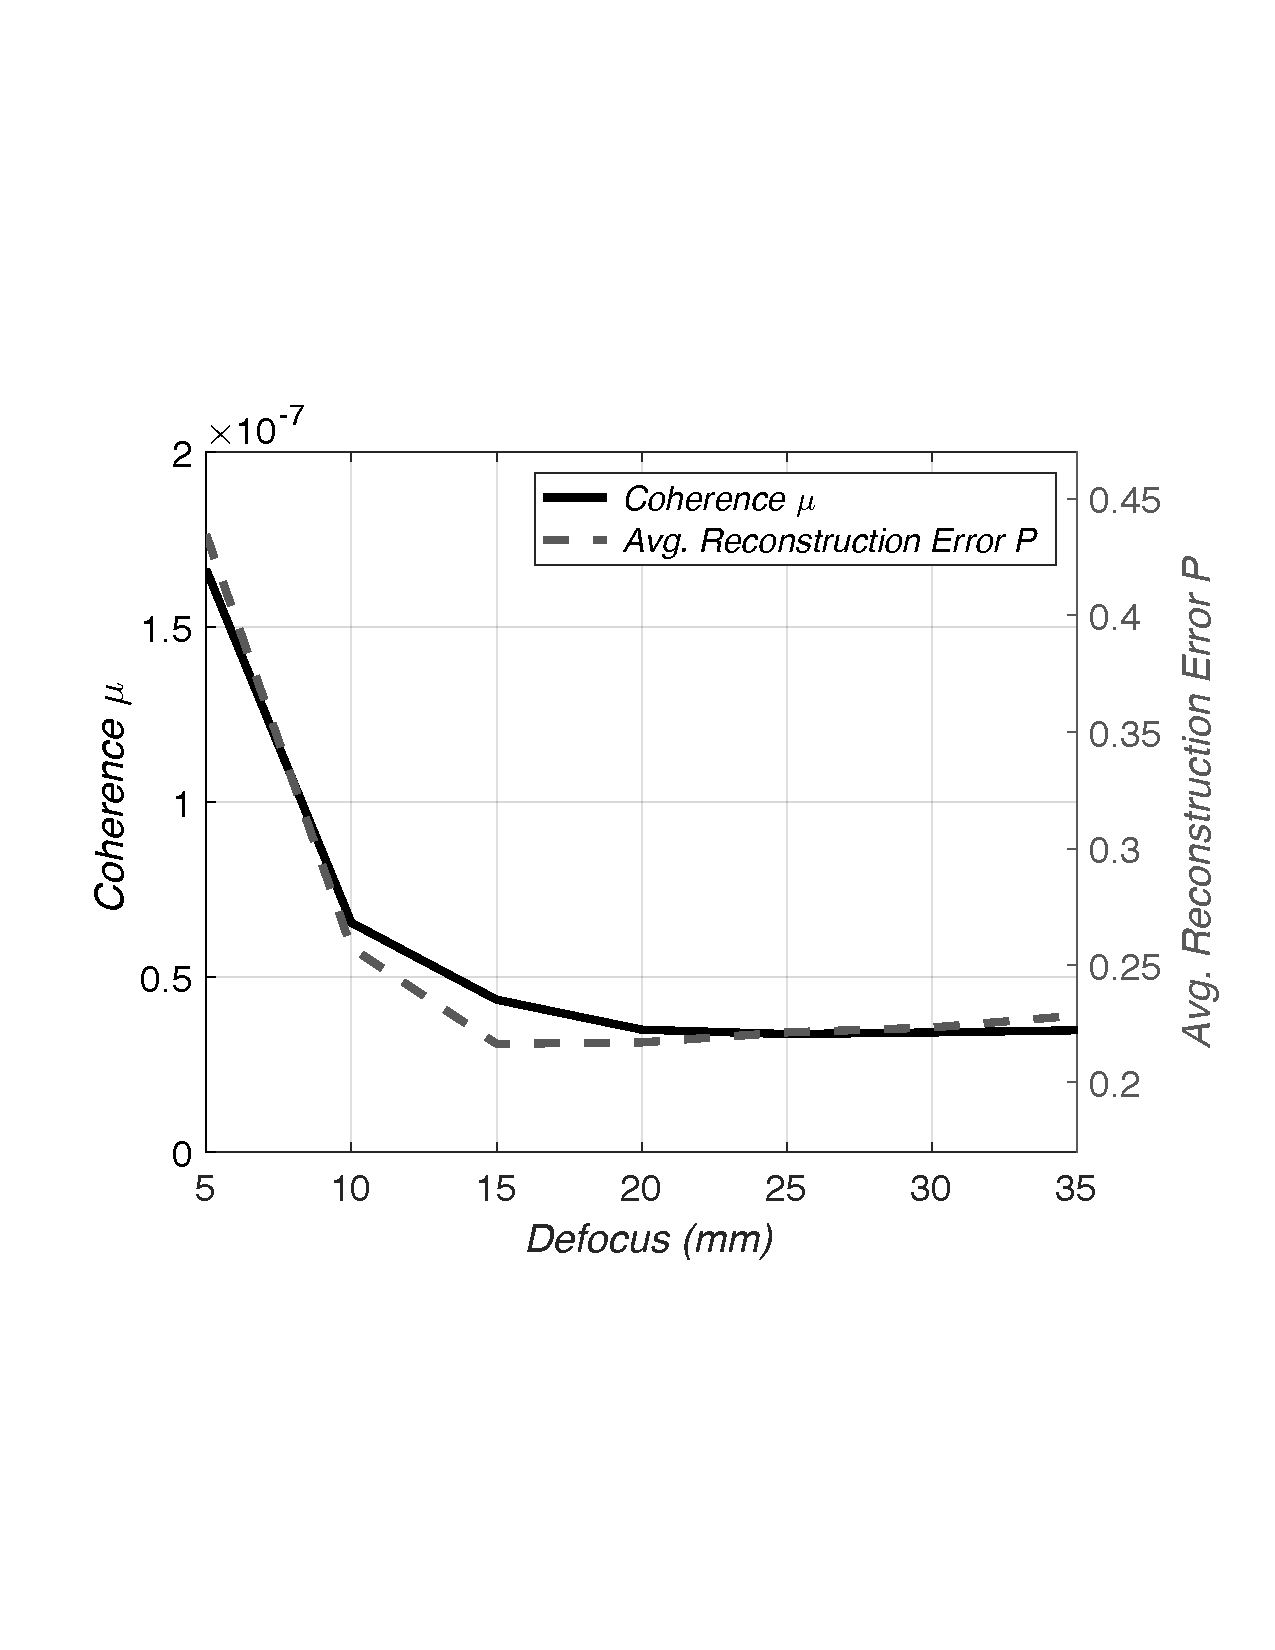
\includegraphics[scale=0.75]{coherenceAndReconErrorVsDefocus}
	\captionof{figure}[The coherence and reconstruction error versus defocus distance.]{The coherence $\mu$ (left vertical axis - black) and reconstruction error P (right vertical axis - dashed gray) plotted as a function of defocus distance $d_im$. }
	\label{fig:coherenceAndReconErrorVsDefocus}
\end{figure}

\begin{figure}[!ht]
	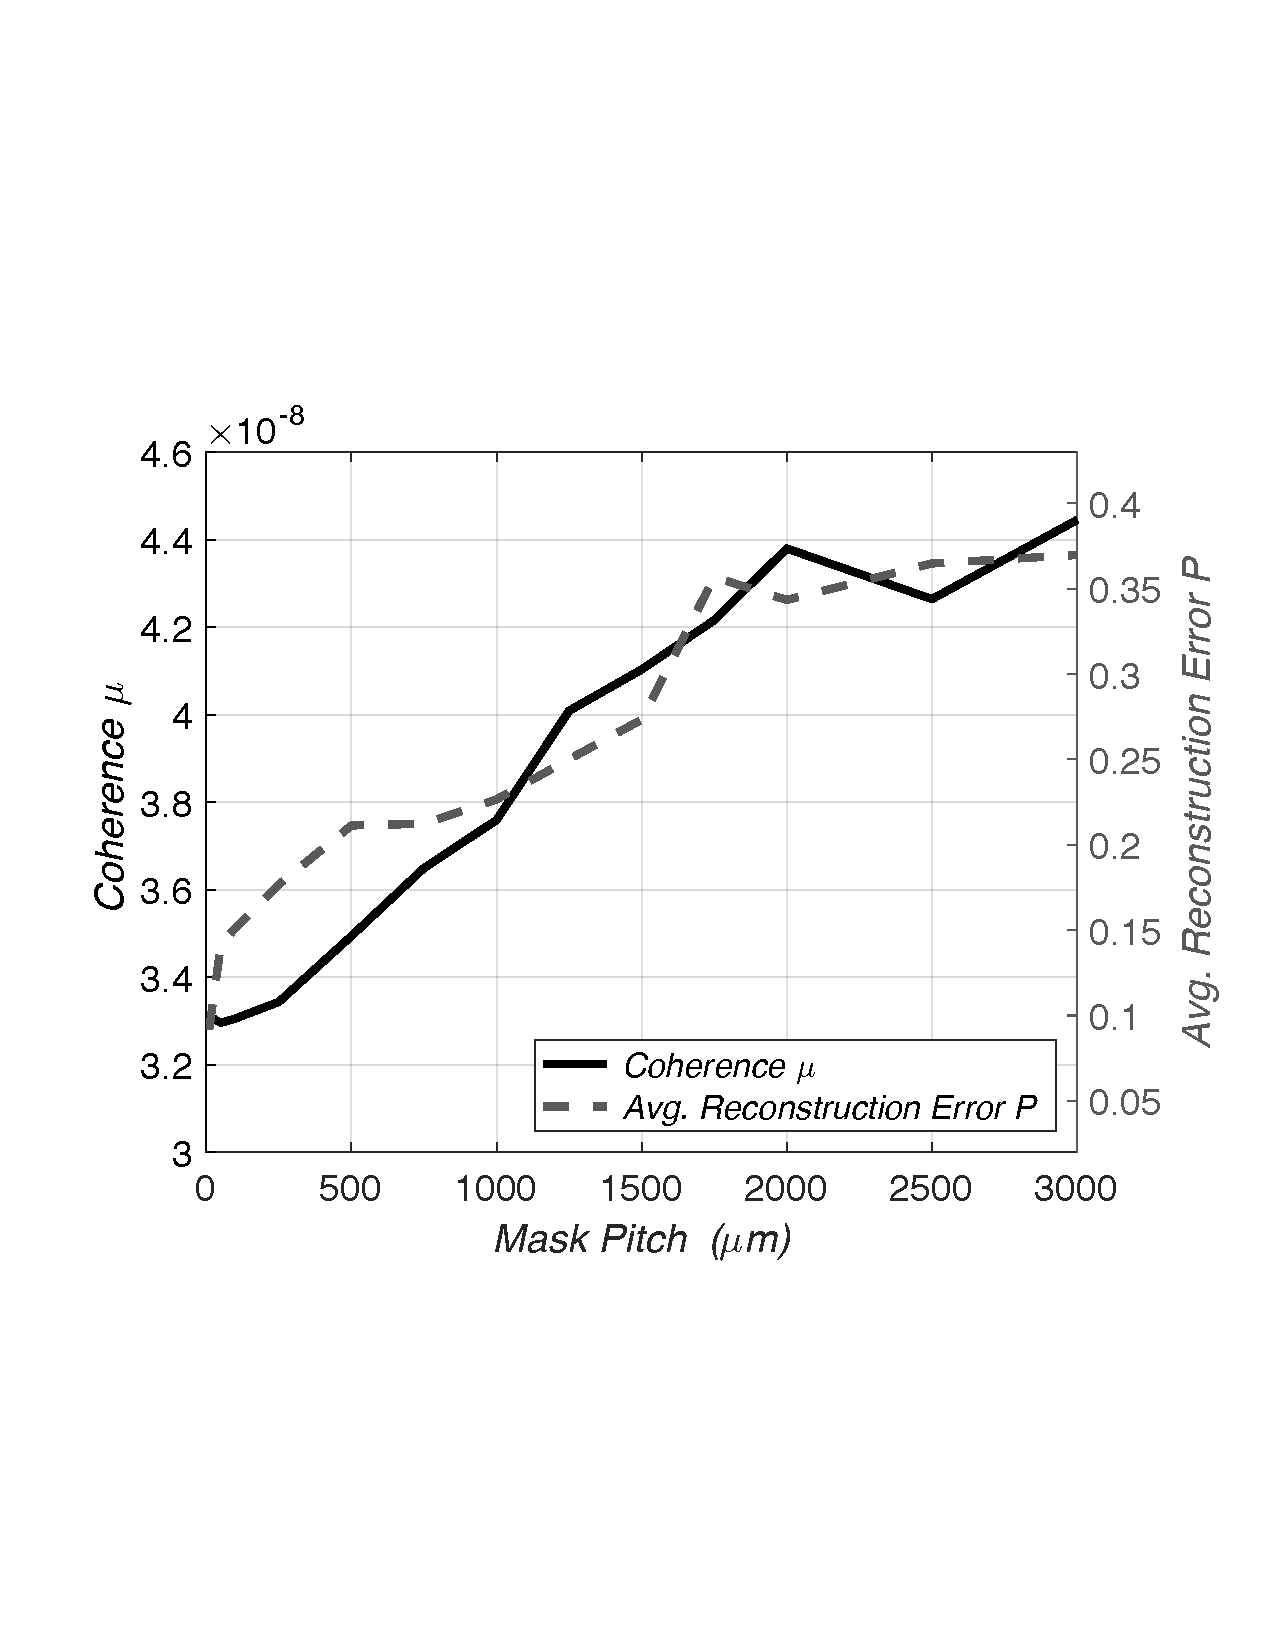
\includegraphics[scale=0.75]{coherenceAndReconErrorVsMaskPitch}
	\captionof{figure}[The coherence and reconstruction error versus pitch of mask 2.]{The coherence $\mu$ (left vertical axis - black) and the reconstruction error P (right vertical axis - dashed gray) is plotted as a function of the pitch of mask 2 }
	\label{fig:coherenceAndReconErrorVsMaskPitch}
\end{figure}


\begin{figure}[!ht]
	\centering
	\includegraphics[scale=0.65]{scoutExpSetup1}
	\captionof{figure}[Photograph of \gls{scout} recording a moving object scene of a black background.]{The camera captures images of scenes displayed on a plasma television approximately 2 meters away..}
	\label{fig:scoutExpSetup1}
\end{figure}

\begin{figure}[!ht]
	\centering
	\includegraphics[scale=0.85]{scoutExpSetup3}
	\captionof{figure}[Photograph of \gls{scout} camera disassembled to show the lens and the first mask.]{The camera disassembled to show the camera body, the optical tube and the custom fabricated lens holder which goes inside the lens tube.}
	\label{fig:scoutExpSetup3}
\end{figure}

To demonstrate the effectiveness of the modified coherence parameter as a predictor of reconstruction error trends, I ran several simulations with complete reconstructions in order to compare reconstruction error to coherence. \Cref{fig:coherenceAndReconErrorVsDefocus} shows that reconstruction error and the coherence parameter follow similar trends for different defocus distances when all other variables are held constant. \Cref{fig:coherenceAndReconErrorVsMaskPitch} shows similar results for varying values of mask pitch $p_2$.

The simulations demonstrate the viability of the architecture and provide an efficient way to optimize most architecture parameter values using the simulated system matrix coherence. Mask throughput cannot currently be optimized because coherence is normalized by full system throughput. The problem of finding optimal mask throughput warrants further investigation.


\section{Experimental Results}\label{sec:ScoutExperimentalResults}

We used a SBIG Model ST-7XMEI CCD camera with modified optics. The object scenes were displayed on a plasma television monitor. Figures \ref{fig:scoutExpSetup1} and \ref{fig:scoutExpSetup3} shows a photograph of the experimental setup. The optical system of the camera includes a 35 mm focal length lens and two random amplitude binary masks. Each mask was printed on transparencies using a high resolution laser printer. Mask 1 has pitch $p1 = 30$ microns and fill factor $F_1 = 0.4$ and is located at a distance $d_{m1} = 14mm$ from the sensor. Mask 2 has pitch $p_2 = 500$ microns and fill factor $F_2 = 0.2$ and is located at a distance $dm2 = 57mm$ from the sensor. These parameters were chosen based on the aforementioned optimization process. A plasma monitor was used because it provides a higher contrast compared to the traditional liquid crystal displays (LCD). However, the black background of the plasma still produced a small amount of irradiance, which is a source of systematic error and potentially reduces the usable amount of dynamic range. 

For our experiment, the captured image resolution $r_x \times r_y$ is $8 \times 8$, while the ground-truth and reconstructed frame differences have a resolution $R_x \times R_y$ of $32 \times 32$. To simulate a low-resolution detector, the camera captures the scenes at $128 \times 128$ sensor pixels and the images are binned down to $8 \times 8$ before being used in reconstruction. 

Experimental results for 29 difference frame sequence is shown in \Cref{app:scoutExpResults}. The object scenes contains two dots (movers) changing position on a black background. Difference frame 1 of this sequence is shown in \Cref{fig:scout_fig10_un}. The top row shows two consecutive, before and after, frames of the scene and the ground-truth difference frame, all at $32 \times 32$ resolution. The bottom row shows the difference of corresponding $8 \times 8$ measurement frames. Finally, the $32 \times 32$ reconstructed difference frame is shown at the bottom right. 

Initially, the amplitude of the movers in the estimated difference frame to did not agree qualitatively with the amplitude of the ground truth difference frame. We realized that this was due to the fact that the exposure time during calibration was not the same as the exposure time during the actual experiment. By normalizing the system matrix obtained during calibration by the ratio of exposure times, we were able to demonstrate quantitative agreement with the ground-truth:

\begin{equation}
	\mb{H}_{recon} = \frac{t_{exp}}{t_{cal}} \mb{H}_{cal}
	\label{eq:ScoutCalibrationMatrixScaling}
\end{equation}

where $t_{exp}$ and $t_{cal}$ are the experiment and calibration exposure times, respectively. This scaling accounts for the physical effect of increased photon collection (and hence photodetector counts) as a function of increased exposure time. The resulting peaks are easily identified against back- ground noise.

\begin{figure}
	\centering
	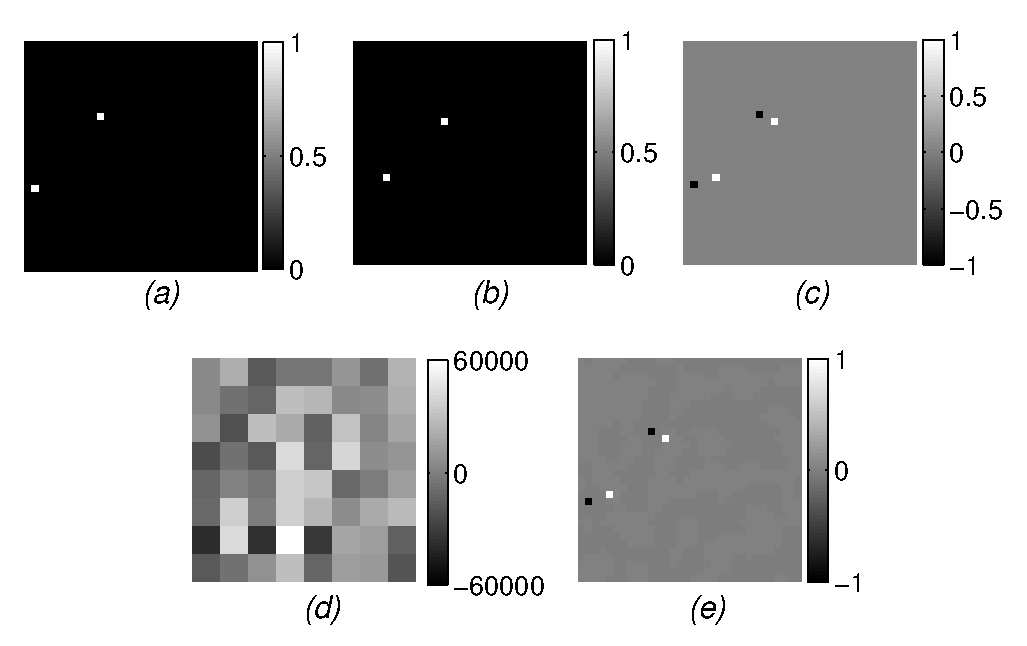
\includegraphics[scale=0.75]{scout_fig10_v2.eps}
	\captionof{figure}[Difference frame 1 of a sequence of two movers on a black background.]{A reconstruction of a $32 \times 32$ scene with two movers of equal amplitude on a black background. (a) ground-truth scene 1 (b) ground-truth scene 2 (c) ground-truth frame difference and (d) measured $8 \times 8$ frame difference, scaled so that it is discernible (e) reconstructed $32 \times 32$ difference frame}
	\label{fig:scout_fig10_un}
\end{figure}

\begin{figure}
	\centering
	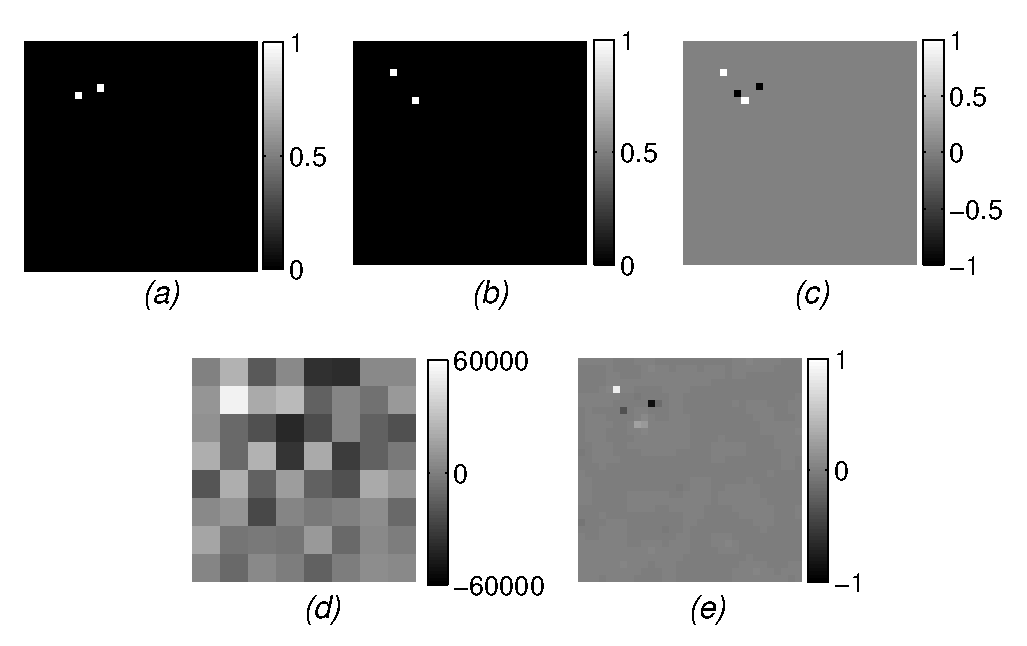
\includegraphics[scale=0.75]{scout_fig11_v2.eps}
	\captionof{figure}[Difference frame 9 of a sequence of two movers on a black background.]{A reconstruction of $32 \times 32$ scene with two movers of equal amplitude on a black background. This frame shows the results when the past and present mover locations are adjacent in the difference frame. (a) ground-truth scene 1 (b) ground-truth scene 2 (c) ground-truth frame difference and (d) measured $8 \times 8$ frame difference, scaled so that it is discernible (e) reconstructed $32 \times 32$ difference frame}
	\label{fig:scout_fig11_un}
\end{figure}


\begin{figure}
	\centering
	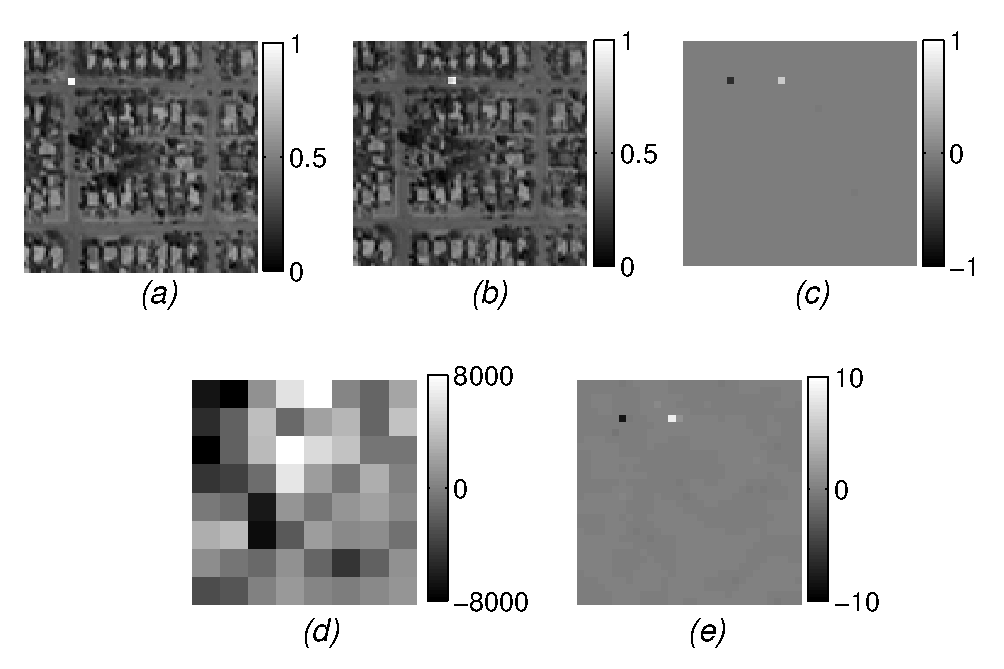
\includegraphics[scale=0.75]{scout_fig12_bg_un}
	\captionof{figure}[Difference frame 1 of a reconstruction video of two movers on a non-zero background.]{Difference frame 1 of a video demonstration of compressive tracking of a  $32 \times 32$ difference scene with a non-zero background. Scene background ©2012 Google. (a) ground- truth scene 1 (b) ground-truth scene 2 (c) ground-truth frame difference and (d) measured $8 \times 8$ frame difference, scaled so that it is discernible (e) reconstructed $32 \times 32$ difference frame}
	\label{fig:scout_fig12_bg_un}
\end{figure}


By inspecting the experimental reconstruction of the 9th difference frame, shown in \Cref{fig:scout_fig11_un}, we note that \gls{scout} reconstructs the amplitude of one or more of the mover locations at a much lower amplitude when compared to the amplitudes in the other reconstructed difference frames. This phenomenon has been correlated to when two locations are adjacent in the ground-truth difference scene. This is an issue that can be traced to the system response matrix H, which is a result of either inaccurate calibrations or through a combination of system design parameters. 


We also performed a more realistic experiment in which a mover simulates an object driving on a street. This demonstrates that the \gls{scout} works well in situations with non-zero backgrounds. This sequence with the results for a single mover is also shown in \Cref{app:scoutExpResults}. The first difference frame of this sequence is shown in \Cref{fig:scout_fig12_bg_un}. As seen in \Cref{fig:scout_fig12_bg_un}(c), the amplitude of the past and present mover locations in the ground-truth are lower than the zero background case. Therefore there is also less contrast in the experimental difference measurements in \Cref{fig:scout_fig12_bg_un}(d), which makes this case more sensitive to noise. 

The most notable feature in the non-zero background results is less quantitative agreement with the ground-truth, even when the calibration matrix is scaled according to \Cref{eq:ScoutCalibrationMatrixScaling}. There are several reasons for this: Nonlinearities in the overall system response that result from a nonlinear monitor “gamma” (mapping from pixel value to output brightness) and inter-pixel interactions that effect brightness. These effects are not captured during calibration as that is performed point-by-point (thus avoiding inter-pixel effects) and with pixels that are fully-on or -off (thus avoiding effects from monitor gamma). Another possible reason is over-multiplexing, since the total light from each frame is increased, there is less dynamic range in the \gls{fpa}, and therefore detector non-linearity be a source of error. Despite the lack of quantitative agreement, qualitative agreement is excellent and the movers are clearly identifiable agains the background in \Cref{fig:scout_fig12_bg_un}(e).



\section{Conclusion}

While the \gls{scout} architecture is well-suited for tracking applications, it does have limitations which make it less useful for general imaging applications. Without sparse scene motion, the priors used in reconstruction will lead to incorrect results. Reconstructions only show the locations of moving objects, and the sensing platform must be stationary relative to the scene so that frame differences are sparse. However, more sophisticated techniques could potentially estimate platform motion and use the additional information to reconstruct the entire scene. Despite its limitations, the architecture is well-suited for applications such as fixed-camera wide-area surveillance where bandwidth and data volume are key concerns.

As discussed earlier in \Cref{chap:Formalism}, many of the theoretical guarantees for \gls{compressive sensing} is not specialized or tuned for the block-circulant system matrix structure exhibited in the \gls{scout} architecture. The problem of reconstructing sparse signals from system matrices with this particular property is not well understood, so further research could yield significant improvements in reconstruction performance. The observed system performance with this algorithm serves to demonstrate the architecture’s viability without the need for significant optimization in the reconstruction stage.

A typical parallel compressive imager would require as many encoding optical elements as simultaneous measurements. The \gls{scout} architecture eliminates this scaling issue by giving up the ability to implement arbitrary projections. Using a pair of masks at different distances to create a block-circulant system matrix, the system makes compressive measurements and reconstructs frame differences. The system can be optimized by adjusting system parameters such as mask pitch and defocus distance. Simulations demonstrated the use of the compressive sensing coherence parameter as an efficient predictor of system matrix performance to jointly optimize these parameters. An experimental system based on the \gls{scout} architecture successfully performed compressive motion tracking on scenes with zero and nonzero backgrounds in most instances. However, the reconstruction of difference scenes with adjacent mover locations caused issues due to the design or calibration of the system matrix. The system showed promising results using a general $\ell_1$-norm minimization algorithm and we believe that further research on sparse reconstruction with block-circulant system matrices may decrease reconstruction error. We also believe that non-isomorphic calibration techniques and adding further degrees of freedom in the design parameters could result in significant performance gains.




